% 第1章第1节：向量的表示（坐标向量、相等、零向量与标准坐标向量）、向量的运算（加法与数乘、线性组合、内积、长度与距离、范数）、向量运算的性质（加法与数乘的性质）。内积与范数的一般性质、夹角与Cauchy--Schwarz不等式见第3章。

\section{向量}
\label{sec:ls-vectors}
\label{sec:ls-objects}
\label{sec:linear-algebra-objects}
\label{sec:linear-algebra-space-representations}
\label{sec:prelim-vectors-matrices}

几次观测的输入是一串数，输出也是一串数；预测减去观测，又得到一串误差。按固定次序排列的一串实数称为向量。本节先规定向量的写法，再定义三类运算：加法与数乘把几个向量合成一个向量，内积把两个向量配成一个数，长度和范数用一个数衡量向量的大小。

\subsection{向量的表示}
\label{sec:ls-vector-representation}
\label{sec:prelim-vector-records}

用向量记录数据，要先说清这串数怎样排列、每个位置记录什么，以及两个向量何时相同。

\paragraph{坐标向量}
$\mathbb R^d$是全部有序$d$元实数组的集合。把其中一个元素的$d$个实数按原有次序竖排成一列，得到实坐标向量（real coordinate vector）：
\[
 \bm u=\begin{pmatrix}u_1\\\vdots\\u_d\end{pmatrix}\in\mathbb R^d,
\]
其中$u_j$是第$j$个坐标，$d$是维数。向量中的一个数只需一个索引$j$就能定位。

\paragraph{列向量与行向量} 本书默认使用列向量。同样的数横排成一行，称为行向量。上标$\top$表示\term{转置}（transpose），它把行向量改写成列向量，也把列向量改写成行向量。因此$(u_1,\ldots,u_d)^\top$就是上面的列向量，正文常用这种写法节省篇幅。

用向量记录数据时，每个位置的含义要事先固定。例如三次观测的（输入，输出）依次为$(1,0)$、$(2,4)$、$(3,6)$。把输入和输出分别排成向量，得到
\[
 \bm x=\begin{pmatrix}1\\2\\3\end{pmatrix},\qquad
 \bm y=\begin{pmatrix}0\\4\\6\end{pmatrix}.
\]
$\bm x$记录输入，$\bm y$记录输出，两个向量的第$i$个位置都对应第$i$次观测。位置的含义一致，后面才能把两个向量逐位置相加或相乘。

\paragraph{相等} 两个向量相等，是指维数相同且对应坐标分别相等。次序是向量的一部分：$(1,2)^\top$与$(2,1)^\top$含有同样的两个数，第一个坐标却不同，所以两者不相等。

\paragraph{零向量} 所有坐标都为零的向量称为零向量，记作$\bm0$。

\paragraph{标准坐标向量} 第$j$个坐标为$1$、其余坐标为$0$的向量记作$\bm e_j$。$\bm e_1,\ldots,\bm e_d$称为$\mathbb R^d$的标准坐标向量，每个$\bm e_j$只“点亮”第$j$个位置。例如在$\mathbb R^3$中，$\bm e_2=(0,1,0)^\top$。

\subsection{加法、数乘与线性组合}
\label{sec:ls-vector-operations}

两个模型各给出一列预测，取平均要用到加法和数乘；把预测和观测相减，得到误差。本小节定义这两种运算及由它们组成的线性组合，再整理它们满足的规则。

\subsubsection{加法与数乘}
\phantomsection
\label{sec:ls-addition-scaling}

同维向量按对应坐标相加减。实数$c$与向量的数乘（scalar multiplication）把每个坐标都乘以$c$。对$\bm x,\bm y\in\mathbb R^d$与$c\in\mathbb R$，对每个$j=1,\ldots,d$，
\begin{equation}
 \begin{gathered}
 (\bm x+\bm y)_j=x_j+y_j,\\
 (\bm x-\bm y)_j=x_j-y_j,\\
 (c\bm x)_j=cx_j.
 \end{gathered}
 \label{eq:ls-vector-addition-scaling}
\end{equation}
特别地，$0\bm x=\bm0$；$-\bm x=(-1)\bm x$称为$\bm x$的相反向量。结果的第$j$个坐标只由输入的第$j$个坐标决定，不同位置的数互不影响，结果仍是$d$维向量。

下面逐坐标计算一组二维向量的加法、减法与数乘。
\begin{example}[向量的加法、减法与数乘]
\label{ex:ls-vector-addition-scaling}
取$\bm x=(1,2)^\top$，$\bm y=(3,-1)^\top$，$\bm z=(1,-3)^\top$与$c=2$。按定义，第一个坐标只和第一个坐标运算，第二个坐标只和第二个坐标运算：
\[
 \begin{aligned}
 \bm x+\bm y&=\begin{pmatrix}1+3\\2+(-1)\end{pmatrix}=\begin{pmatrix}4\\1\end{pmatrix},\\
 \bm x-\bm y&=\begin{pmatrix}1-3\\2-(-1)\end{pmatrix}=\begin{pmatrix}-2\\3\end{pmatrix},\\
 c\bm z&=\begin{pmatrix}2\cdot1\\2\cdot(-3)\end{pmatrix}=\begin{pmatrix}2\\-6\end{pmatrix}.
 \end{aligned}
\]
三个结果仍是二维向量。例如$\bm x+\bm y$的第二个坐标$1$只来自$\bm x$与$\bm y$的第二个坐标$2$和$-1$，与第一个坐标的取值无关。
\end{example}

两个向量相加，要求维数相同，还要求对应位置的含义相同。维数不同时，坐标无法逐位置配对，加法没有定义。维数相同而位置含义不同时，逐坐标相加仍能算出数，但结果没有意义。

\subsubsection{线性组合}

把加法和数乘结合起来：若干同维向量分别乘以系数后相加，得到
\begin{equation}
 c_1\bm v_1+c_2\bm v_2+\cdots+c_k\bm v_k=\sum_{j=1}^k c_j\bm v_j,
 \label{eq:ls-linear-combination}
\end{equation}
称为$\bm v_1,\ldots,\bm v_k$的一个\term{线性组合}（linear combination），$c_1,\ldots,c_k$称为系数。

结果的第$i$个坐标是
\[
 \Bigl(\sum_{j=1}^k c_j\bm v_j\Bigr)_i=\sum_{j=1}^k c_j(\bm v_j)_i,
\]
即各向量在第$i$个位置上的坐标按同一组系数加权求和。系数可以是任意实数，不要求非负，也不要求和为$1$。

用线性组合可以一次写出全部预测误差。下面回到前面的三次观测。
\begin{example}[残差向量是线性组合]
\label{ex:ls-residual-vector}
输入与输出仍是$\bm x=(1,2,3)^\top$与$\bm y=(0,4,6)^\top$。若用输入的$w$倍预测输出，三次预测排在一起就是数乘$w\bm x$。再逐位置减去观测，得到残差向量（residual vector）
\[
 \bm r=w\bm x-\bm y=w\bm x+(-1)\bm y,
\]
它是$\bm x,\bm y$以$w$和$-1$为系数的线性组合。例如取$w=1$，
\[
 \bm r=\begin{pmatrix}1-0\\2-4\\3-6\end{pmatrix}=\begin{pmatrix}1\\-2\\-3\end{pmatrix}.
\]
$\bm r$的第$i$个坐标正是第$i$次观测的预测误差。三个误差不必逐次另算，一个线性组合就把它们同时写了出来。
\end{example}

下一个例子将贯穿线性空间各章。它用线性组合说明，两个特征的取值向量可能只相差一个很短的向量。
\begin{example}[贯穿例：两个几乎相同的特征]
\label{ex:ls-nearly-collinear-features}
设三个样本上有两个特征，取值向量分别是$\bm c_1$与$\bm c_2$；另取辅助向量$\bm q$：
\[
 \bm c_1=\begin{pmatrix}1\\1\\1\end{pmatrix},\qquad
 \bm c_2=\begin{pmatrix}1\\1+\varepsilon\\1-\varepsilon\end{pmatrix},\qquad
 \bm q=\begin{pmatrix}0\\1\\-1\end{pmatrix},
\]
其中$\varepsilon$是一个实参数。第一个特征在三个样本上都取$1$；第二个特征在第一个样本上也取$1$，在后两个样本上分别多出$\varepsilon$和少了$\varepsilon$。$\bm q$恰好记录了这种偏离的模式，逐坐标计算可得
\[
 \bm c_1+\varepsilon\bm q=\begin{pmatrix}1+0\\1+\varepsilon\\1-\varepsilon\end{pmatrix}=\bm c_2.
\]
于是$\bm c_2=\bm c_1+\varepsilon\bm q$，第二个特征的取值向量是$\bm c_1$与$\bm q$以$1$和$\varepsilon$为系数的线性组合。$|\varepsilon|$很小时，两者只相差短向量$\varepsilon\bm q$，几乎是同一串数。
\end{example}
说两个向量的方向“几乎相同”，需要先有夹角的概念；第~\ref{sec:ls-inner-product-definition}节用内积定义夹角以后再说明。

\subsubsection{加法与数乘的性质}
\label{sec:ls-vector-operation-rules}

加法与数乘是逐坐标定义的，只用到实数的加法与乘法。因此下面每一条规则，都可以在任一坐标上用实数运算直接验证。设$\bm u,\bm v,\bm w\in\mathbb R^d$，$a,b\in\mathbb R$。

\paragraph{加法交换律与结合律}
\[
 \begin{gathered}
 \bm u+\bm v=\bm v+\bm u,\\
 (\bm u+\bm v)+\bm w=\bm u+(\bm v+\bm w).
 \end{gathered}
\]

\paragraph{零向量与相反向量}
\[
 \begin{gathered}
 \bm u+\bm0=\bm u,\\
 \bm u+(-\bm u)=\bm0.
 \end{gathered}
\]

\paragraph{数乘结合律与单位数}
\[
 \begin{gathered}
 a(b\bm u)=(ab)\bm u,\\
 1\bm u=\bm u.
 \end{gathered}
\]

\paragraph{分配律}
\[
 \begin{gathered}
 (a+b)\bm u=a\bm u+b\bm u,\\
 a(\bm u+\bm v)=a\bm u+a\bm v.
 \end{gathered}
\]

有了这八条规则，有限次加法与数乘可以任意加括号、交换加项次序并展开，结果不变；线性组合因此可以像多项式一样合并同类项。下一节的同形矩阵、第~\ref{sec:ls-tensors-objects}节的多维数组也逐项相加与数乘，同样的验证对它们照样成立。第~\ref{chap:linear-representation}章将看到，后面许多结论只依赖这八条规则，而不依赖对象是一列数还是一张表。

\subsection{内积}

加法与数乘的结果仍是向量。数据分析还常要把两个向量配成一个数，或用一个数衡量一个向量的大小。本小节给出欧氏内积，并由它得到长度与距离；下一小节再介绍衡量大小的其他方式，即范数。内积的一般理论在第~\ref{chap:inner-product-spaces}章建立。

\subsubsection{内积的定义}
\phantomsection
\label{sec:ls-inner-products}
\label{sec:prelim-vector-inner-length}

线性预测对一次观测的输入$x_1,\ldots,x_d$和一组权重$w_1,\ldots,w_d$计算加权和$\sum_jx_jw_j$，即两串数逐项相乘再相加。

这种运算单独定义如下：对$\bm x,\bm y\in\mathbb R^d$，标准坐标下的欧氏内积为
\begin{equation}
 \langle\bm x,\bm y\rangle
 =\sum_{j=1}^d x_jy_j,
 \label{eq:ls-euclidean-inner-product}
\end{equation}
也写作$\bm x^\top\bm y$。输入是两个同维向量，输出是一个标量。第~\ref{sec:ls-matrices}节将说明，$\bm x^\top\bm y$正是$1\times d$矩阵与$d\times1$矩阵的乘积。

内积为零的情形有专门的名称：$\langle\bm x,\bm y\rangle=0$时，称两向量\term{正交}（orthogonal）。下面先计算一个内积，再检查平面上两对向量是否正交。
\begin{example}[内积与正交的计算]
\label{ex:ls-inner-product-orthogonality}
在$\mathbb R^2$中取三对向量：$(2,-1)^\top$与$(3,4)^\top$，标准坐标向量$\bm e_1=(1,0)^\top$与$\bm e_2=(0,1)^\top$，以及$(1,1)^\top$与$(1,-1)^\top$。对每一对都按定义逐项相乘再相加：
\[
 \begin{gathered}
 \left\langle\begin{pmatrix}2\\-1\end{pmatrix},\begin{pmatrix}3\\4\end{pmatrix}\right\rangle=2\cdot3+(-1)\cdot4=2,\\
 \langle\bm e_1,\bm e_2\rangle=\left\langle\begin{pmatrix}1\\0\end{pmatrix},\begin{pmatrix}0\\1\end{pmatrix}\right\rangle=1\cdot0+0\cdot1=0,\\
 \left\langle\begin{pmatrix}1\\1\end{pmatrix},\begin{pmatrix}1\\-1\end{pmatrix}\right\rangle=1\cdot1+1\cdot(-1)=0.
 \end{gathered}
\]
第一对的内积为$2$，不正交；后两对的内积为零，因而正交。画在平面上，$\bm e_1,\bm e_2$沿两条坐标轴，$(1,1)^\top,(1,-1)^\top$沿两条对角线，两对确实都互相垂直。
\end{example}
在平面上，正交恰好就是垂直。一般维数下为什么也可以这样理解，要等第~\ref{sec:ls-inner-product-definition}节定义夹角以后才能说明。

\subsubsection{长度与距离}
\phantomsection
\label{sec:linear-algebra-length-angle-distance}

向量与自身的内积$\langle\bm x,\bm x\rangle=\sum_jx_j^2$是各坐标的平方和，总是非负，可以开平方。开平方后得到向量的长度
\begin{equation}
 \lVert\bm x\rVert=\sqrt{\langle\bm x,\bm x\rangle}.
 \label{eq:linear-algebra-inner-product-norm}
\end{equation}
由标准内积给出的长度称为欧氏范数（Euclidean norm）或$2$范数，记作
\[
 \lVert\bm x\rVert_2=\sqrt{\sum_{j=1}^d x_j^2}.
\]
它把平面上的勾股定理推广到$d$个坐标。

长度为$1$的向量称为单位向量。非零向量$\bm x$除以自身长度，得到$\bm x/\lVert\bm x\rVert_2$。它的各坐标平方和为$1$，是一个单位向量；它与$\bm x$方向相同，只是去掉了大小。

两点之间的距离用差向量的长度衡量：$\bm x$与$\bm y$的欧氏距离定义为$\lVert\bm x-\bm y\rVert_2$。

下面计算前面残差向量的长度，以及平面上两点的距离。
\begin{example}[长度与距离的计算]
\label{ex:ls-length-distance}
先回到示例~\ref{ex:ls-residual-vector}中$w=1$时的残差$\bm r=(1,-2,-3)^\top$，计算它长度的平方；再计算平面上两点$(1,2)^\top$与$(4,6)^\top$之差的长度。按定义逐坐标平方再相加：
\[
 \begin{gathered}
 \lVert\bm r\rVert_2^2=1^2+(-2)^2+(-3)^2=14,\\
 \left\lVert\begin{pmatrix}1\\2\end{pmatrix}-\begin{pmatrix}4\\6\end{pmatrix}\right\rVert_2=\sqrt{(-3)^2+(-4)^2}=5.
 \end{gathered}
\]
$\bm r$的各坐标是三次观测的预测误差，所以$\lVert\bm r\rVert_2^2=14$正是$w=1$时的平方误差总和。

第二个算式中，差向量的两个坐标$-3,-4$是直角三角形的两条直角边，距离$5$就是勾股定理给出的斜边长。
\end{example}
用距离比较实际数据时，应先约定各坐标的单位和尺度，否则数值大的坐标会支配距离。

\subsection{范数}
\label{sec:ls-coordinate-norms}

\subsubsection{范数的定义}

欧氏长度先把各坐标平方再相加。衡量向量大小还有别的做法：可以累加各坐标的绝对值，也可以只看最大的绝对值。这些大小度量统称为范数，适合衡量不同含义的误差。

有限维中最常用的是$p$范数：
\begin{equation}
 \begin{gathered}
 \lVert\bm x\rVert_p=\left(\sum_j|x_j|^p\right)^{1/p}\quad(1\leq p<\infty),
 \\
 \lVert\bm x\rVert_\infty=\max_j|x_j|.
 \end{gathered}
 \label{eq:ls-p-norm}
\end{equation}
$p=1$时累加绝对偏差；$p=2$时累加平方偏差再开方，就是欧氏长度；$p=\infty$时取最大的坐标偏差。

下面在同一个向量上比较这三种范数。
\begin{example}[三种$p$范数的计算]
\label{ex:ls-p-norms}
取$\bm x=(3,-4)^\top$，分别按三种方式汇总它的两个坐标：
\[
 \begin{gathered}
 \lVert\bm x\rVert_1=|3|+|-4|=7,\\
 \lVert\bm x\rVert_2=\sqrt{3^2+(-4)^2}=5,\\
 \lVert\bm x\rVert_\infty=\max\{|3|,|-4|\}=4.
 \end{gathered}
\]
同一个向量在三种范数下的大小依次为$7$、$5$、$4$。

$1$范数把两个绝对偏差全部累加，$\infty$范数只记最大的那个，$2$范数介于两者之间。所以说一个向量“有多大”，要先说明用的是哪种范数。
\end{example}

不同的范数也给出不同形状的单位球$\{\bm x:\lVert\bm x\rVert\leq1\}$，图~\ref{fig:ls-norm-unit-balls}把三种单位球并排比较。这些范数共同满足的性质在下一小节证明。

\begin{figure*}[htbp]
  \centering
  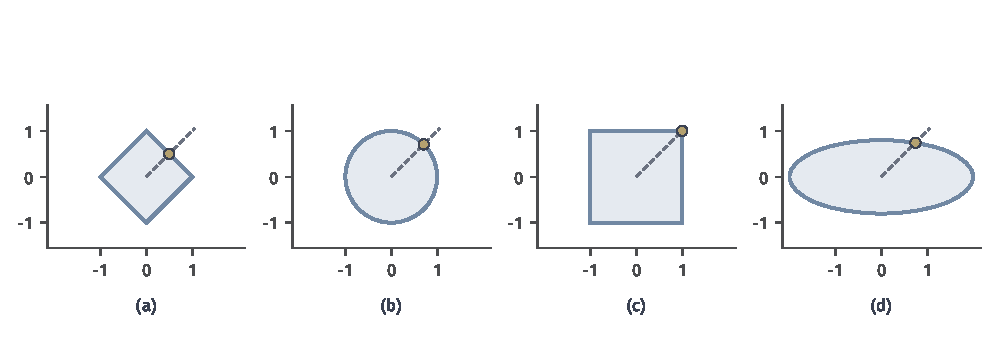
\includegraphics[width=169mm]{figures/00-shared/mathematical-preliminaries-upper/02-linear-spaces/matplotlib/ls-norm-unit-balls/ls-norm-unit-balls.pdf}
  \caption{三种范数的单位球。左：$\ell_1$单位球为菱形（累加绝对偏差）；中：$\ell_2$单位球为圆（欧氏长度）；右：$\ell_\infty$单位球为正方形（最大坐标偏差）。同一个点$(1,1)$的三种范数依次为$2$、$\sqrt2$、$1$。三者之间的倍数关系见第~\ref{sec:ls-error-scale-comparison}节。三图坐标尺度相同，为解析教学例。}
  \label{fig:ls-norm-unit-balls}
\end{figure*}

\subsubsection{范数的性质}
\label{sec:ls-p-norm-properties}

$1$、$2$、$\infty$范数的算法不同，却有几条共同的性质：大小非负，只有零向量的大小为零；向量放大$c$倍，大小变为$|c|$倍；两个向量之和的大小不超过各自大小之和。本小节对全部$p$范数证明这些性质，再比较不同$p$范数给出的大小最多相差多少倍。

\paragraph{非负性、正定性与齐次性}
这三条可以从公式直接读出。$\lVert\bm x\rVert_p$由绝对值汇总而成，总是非负；它为零当且仅当每个$|x_j|=0$，即$\bm x=\bm0$。

把$\bm x$换成$c\bm x$，每个$|x_j|$都乘以$|c|$。在$1\leq p<\infty$时，公式中的$p$次方与$1/p$次方相互抵消；在$p=\infty$时，最大值也乘以$|c|$。所以
\[
 \lVert c\bm x\rVert_p=|c|\,\lVert\bm x\rVert_p.
\]

\paragraph{三角不等式}
需要证明的只有三角不等式$\lVert\bm x+\bm y\rVert_p\leq\lVert\bm x\rVert_p+\lVert\bm y\rVert_p$。$p=1$和$p=\infty$时，它由实数的三角不等式逐坐标得到，见下面Minkowski不等式的证明。

$1<p<\infty$时，三角不等式要借助Hölder不等式。它用一对$p$范数与$q$范数控制两个向量逐坐标乘积之和，两个指数须满足共轭条件$1/p+1/q=1$。
\begin{theorem}[有限维Hölder不等式]
\label{thm:linear-algebra-holder}
设$\bm x,\bm y\in\mathbb R^d$，$1\leq p,q\leq\infty$且$1/p+1/q=1$（约定$1/\infty=0$），则
\begin{equation}
 |\bm x^\top\bm y|\leq\lVert\bm x\rVert_p\lVert\bm y\rVert_q.
 \label{eq:linear-algebra-holder}
\end{equation}
\end{theorem}
\begin{proof}
先设$1<p,q<\infty$，分三步证明。

第一步，证明Young不等式：对$u,v\geq0$，
\[
 uv\leq\frac{u^p}{p}+\frac{v^q}{q}.
\]
$u=0$时左侧为零，不等式成立。$u>0$时令$t=v/u^{p-1}\geq0$。由$1/p+1/q=1$得$(p-1)q=p$，于是
\[
 v^q=t^qu^{(p-1)q}=t^qu^p,\qquad uv=tu^p.
\]
代入后，不等式化为
\[
 u^p\Bigl(\frac1p+\frac{t^q}{q}-t\Bigr)\geq0.
\]
只需证明括号内的函数$f(t)=1/p+t^q/q-t$在$t\geq0$上非负。它的导数
\[
 f'(t)=t^{q-1}-1
\]
在$0<t<1$时为负、在$t>1$时为正，所以$f$在$t\geq0$上的最小值是
\[
 f(1)=\frac1p+\frac1q-1=0,
\]
不等式成立。

第二步，在单位尺度下求和。若$\bm x$或$\bm y$为零向量，结论两侧都为零。否则令$u_j=|x_j|/\lVert\bm x\rVert_p$、$v_j=|y_j|/\lVert\bm y\rVert_q$，则
\[
 \sum_ju_j^p=\sum_jv_j^q=1.
\]
对每个$j$用Young不等式再求和，得
\[
 \sum_ju_jv_j\leq\frac1p\sum_ju_j^p+\frac1q\sum_jv_j^q=\frac1p+\frac1q=1.
\]

第三步，恢复尺度。上式两边乘以$\lVert\bm x\rVert_p\lVert\bm y\rVert_q$，再用$|\bm x^\top\bm y|\leq\sum_j|x_j||y_j|$，即得
\[
 |\bm x^\top\bm y|\leq\sum_j|x_j||y_j|\leq\lVert\bm x\rVert_p\lVert\bm y\rVert_q.
\]

端点情形直接估计。$p=1$、$q=\infty$时，
\[
 \sum_j|x_j||y_j|\leq\Bigl(\max_j|y_j|\Bigr)\sum_j|x_j|=\lVert\bm x\rVert_1\lVert\bm y\rVert_\infty;
\]
$p=\infty$、$q=1$时交换两个向量的角色。
\end{proof}
$p=q=2$时，它给出$|\bm x^\top\bm y|\leq\lVert\bm x\rVert_2\lVert\bm y\rVert_2$。第~\ref{sec:ls-inner-product-definition}节将只用内积公理，对任一内积证明同样形式的不等式，即Cauchy--Schwarz不等式。

有了Hölder不等式，就可以对一般的$p$证明三角不等式。做法是把$|x_j+y_j|^p$拆成两个乘积之和，再对每一部分使用Hölder不等式。
\begin{theorem}[有限维Minkowski不等式]
\label{thm:linear-algebra-minkowski}
设$\bm x,\bm y\in\mathbb R^d$，$1\leq p\leq\infty$，则
\begin{equation}
 \lVert\bm x+\bm y\rVert_p\leq\lVert\bm x\rVert_p+\lVert\bm y\rVert_p.
 \label{eq:linear-algebra-minkowski}
\end{equation}
\end{theorem}
\begin{proof}
先处理两个端点。$p=1$时，对每个坐标使用实数的三角不等式，再求和，得到
\[
 \sum_j|x_j+y_j|\leq\sum_j|x_j|+\sum_j|y_j|.
\]
$p=\infty$时，对每个$j$都有
\[
 |x_j+y_j|\leq\lVert\bm x\rVert_\infty+\lVert\bm y\rVert_\infty.
\]
左侧对$j$取最大值，就得到所需结论。

下面设$1<p<\infty$。若$\bm x+\bm y=\bm0$，左侧为零，结论成立；以下设和向量非零。

取$q=p/(p-1)$，则$1/p+1/q=1$。先把每个坐标的$p$次方拆开，再用实数的三角不等式：
\[
 \begin{aligned}
 |x_j+y_j|^p
 &=|x_j+y_j|^{p-1}|x_j+y_j|\\
 &\leq |x_j+y_j|^{p-1}(|x_j|+|y_j|).
 \end{aligned}
\]
令$s_j=|x_j+y_j|^{p-1}$，把这些数排成向量$\bm s$。由于$(p-1)q=p$，它的$q$范数为
\[
 \begin{aligned}
 \lVert\bm s\rVert_q
 &=\Bigl(\sum_j|x_j+y_j|^p\Bigr)^{1/q}\\
 &=\lVert\bm x+\bm y\rVert_p^{p-1}.
 \end{aligned}
\]
把逐坐标的不等式求和，并对含$|x_j|$和含$|y_j|$的两部分分别使用Hölder不等式，得到
\[
 \begin{aligned}
 \lVert\bm x+\bm y\rVert_p^p
 &\leq\sum_js_j|x_j|+\sum_js_j|y_j|\\
 &\leq\lVert\bm s\rVert_q
       \bigl(\lVert\bm x\rVert_p+\lVert\bm y\rVert_p\bigr)\\
 &=\lVert\bm x+\bm y\rVert_p^{p-1}
       \bigl(\lVert\bm x\rVert_p+\lVert\bm y\rVert_p\bigr).
 \end{aligned}
\]
两边除以正数$\lVert\bm x+\bm y\rVert_p^{p-1}$，即得结论。
\end{proof}
所以每个$p$范数都满足三角不等式，特别是欧氏长度：两边之和不小于第三边。


\paragraph{范数的比较}
\phantomsection
\label{sec:ls-error-scale-comparison}

不同的$p$范数给同一个向量的大小不同。误差估计常常要在两种范数之间换算，因此需要知道它们最多相差多少倍。对$\mathbb R^d$中的坐标范数，这个倍数可以由有限求和直接算出。
\begin{theorem}[坐标范数的比较]
\label{thm:ls-coordinate-norm-comparison}
设$1\leq p\leq q\leq\infty$，约定$1/\infty=0$。对$\bm x\in\mathbb R^d$，
\begin{equation}
 \lVert\bm x\rVert_q\leq\lVert\bm x\rVert_p\leq d^{1/p-1/q}\lVert\bm x\rVert_q.
 \label{eq:ls-coordinate-norm-comparison}
\end{equation}
\end{theorem}
\begin{proof}
$\bm x=\bm0$时三项都为零，下设$\bm x\neq\bm0$。

左侧。令$\bm u=\bm x/\lVert\bm x\rVert_p$，则$\lVert\bm u\rVert_p=1$，所以每个$|u_j|\leq1$。$q=\infty$时这就是$\lVert\bm u\rVert_\infty\leq1$。

$q<\infty$时，由$|u_j|\leq1$与$q\geq p$得$|u_j|^q\leq|u_j|^p$。对$j$求和，得
\[
 \lVert\bm u\rVert_q^q\leq\lVert\bm u\rVert_p^p=1.
\]
两种情形都有$\lVert\bm u\rVert_q\leq1$，两边乘以$\lVert\bm x\rVert_p$即得。

右侧。$p=q$时两侧相同。$q=\infty$时，每一项$|x_j|^p$都不超过$\lVert\bm x\rVert_\infty^p$，于是
\[
 \sum_j|x_j|^p\leq d\,\lVert\bm x\rVert_\infty^p,
\]
开$p$次方即得。

设$p<q<\infty$，取$r=q/p>1$，其共轭指数满足$1/r'=1-p/q$。对向量$(|x_1|^p,\ldots,|x_d|^p)^\top$与全$1$向量使用Hölder不等式（定理~\ref{thm:linear-algebra-holder}），得
\[
 \begin{aligned}
 \sum_j|x_j|^p\cdot1
 &\leq\Bigl(\sum_j|x_j|^{q}\Bigr)^{p/q}d^{\,1-p/q}\\
 &=\lVert\bm x\rVert_q^p\,d^{\,1-p/q}.
 \end{aligned}
\]
两边开$p$次方，得
\[
 \lVert\bm x\rVert_p\leq d^{1/p-1/q}\lVert\bm x\rVert_q.
\]
\end{proof}
最常用的是$p,q\in\{1,2,\infty\}$的情形：
\[
 \begin{gathered}
 \lVert\bm x\rVert_\infty\leq\lVert\bm x\rVert_2\leq\sqrt d\,\lVert\bm x\rVert_\infty,\\
 \lVert\bm x\rVert_2\leq\lVert\bm x\rVert_1\leq\sqrt d\,\lVert\bm x\rVert_2,\\
 \lVert\bm x\rVert_\infty\leq\lVert\bm x\rVert_1\leq d\,\lVert\bm x\rVert_\infty.
 \end{gathered}
\]
下面在示例~\ref{ex:ls-p-norms}的向量上核对前两行。
\begin{example}[范数比较的数值核对]
\label{ex:ls-norm-comparison-check}
取$d=2$与$\bm x=(3,-4)^\top$。示例~\ref{ex:ls-p-norms}已经算出$\lVert\bm x\rVert_1=7$，$\lVert\bm x\rVert_2=5$，$\lVert\bm x\rVert_\infty=4$。代入前两行，比较常数分别为$\sqrt2$：
\[
 \begin{gathered}
 4\leq5\leq4\sqrt2\approx5.66,\\
 5\leq7\leq5\sqrt2\approx7.07.
 \end{gathered}
\]
四个不等式都成立，而且右侧的界离实际值不远。同一个误差$\bm x$在三种范数下读出$4$、$5$、$7$三个不同的数，比较定理保证的是这些读数之间的倍数不超过与维数有关的常数。
\end{example}
两侧的常数一般都不能改进，取等号的向量很简单。
\begin{example}[比较常数的取等]
\label{ex:ls-l1-linf-constants}
两个极端的向量分别使两侧取等号：只有一个非零坐标的$\bm e_1$，和各坐标一样大的全$1$向量$\bm 1$。

对每个$p$都有$\lVert\bm e_1\rVert_p=1$，所以$\bm e_1$使左侧取等号。

另一方面，全$1$向量的各范数为
\[
 \lVert\bm 1\rVert_p=d^{1/p}\quad(p<\infty),\qquad
 \lVert\bm 1\rVert_\infty=1.
\]
因此在约定$1/\infty=0$下总有
\[
 \lVert\bm 1\rVert_p=d^{1/p-1/q}\lVert\bm 1\rVert_q,
\]
右侧取等号。

大小全部集中在一个坐标上时，各范数读数相同；各坐标绝对值相等时，读数相差最大。例如$\ell_1$与$\ell_\infty$之间的常数$1$与$d$分别由$\bm e_1$和$\bm 1$达到，都不能改进。
\end{example}
右侧的常数随维数增长。维数较大时，换用范数带来的倍数差别不能在误差估计中忽略；固定维数下的比较式也不能当作对所有维数一致成立的界。

这里只比较了有明确公式的坐标范数。有限维空间上任意两个范数都只相差常数倍（定理~\ref{thm:ls-norm-equivalence}），这一结论的证明要用到闭有界集上连续函数的最值，在第~\ref{sec:multivariable-norm-equivalence}节给出。

本节建立了坐标向量的基本计算：加法、数乘与线性组合产生新的向量，欧氏内积把两个向量配成一个数，范数衡量向量的大小，满足非负性、正定性、齐次性与三角不等式，不同$p$范数之间只差与维数有关的常数倍。把若干向量并排放在一起，就得到下一节的矩阵。
